\chapter{Introduction}
{%\hypersetup{linkcolor=black}
\startcontents[chapters]
\printcontents[chapters]{}{1}{}
}

\noindent\\
This project will detail the design, implementation, and verification, of a new multi-core RISC processor aimed at FPGA devices. This project was chosen due to my interest in processor design, in which I have only previously designed single-core RISC processors, and wish to extend this knowledge to gain a basic understanding of multi-core communication, design considerations, and the challenges of software and hardware parallelism first hand.

I will use this opportunity to further develop my knowledge of FPGA and processor design by implementing, designing, and verifying, a multi-core RISC processor from scratch, including the design of a communication interface between multiple cores.

\section{Why Multi-core?}

Moore's Law states that the number of transistors in a chip will double every 2 years \cite{}. CPU designers would utilize the  additional transistors to add more pipeline stages in the processor to reduce the propagation delay \cite{} which would allow for higher clock frequencies. 

%This would allow the processor to be run at higher clock frequencies as the logic between pipeline stages is reduced. The faster clock frequency would result in computational performance because more instructions could be executed in a period of time.

The size of transistors have been decreasing \cite{} and today can be manufactured in sub-10 nanometer range. However, the extremely small transistor size increases electrical leakage and other negative effects resulting in unreliability and potential damage to the transistor \cite{}.  The high transistor count produces large amounts of heat and requires increasing power to supply the chip. These trade-offs are currently managed by reducing the input voltage, utilising complex cooling techniques, and reducing clock frequency. These factors limit the performance of the chip significantly.
These are contributing factors to Moore's Law \textit{slowing} down. 
The capacity limit of the current-generation planar transistors is approaching and so in order for performance increases to continue, other approaches such as alternate transistor technologies like Multigate transistors \cite{subramanian2010multiple}, software and hardware optimisations, and multi-processor architectures are employed.

This report will focus on the latter: to produce a small multi-core processor that can utilise software-based parallelism to gain performance benefits, compared to a larger single-core design.

\section{Why RISC?}
RISC architectures feature simpler and fewer instructions compared to CISC, which emphasises instructions that perform larger tasks. A single CISC instruction might be performed with multiple RISC instructions. Because of the fewer and simpler instructions, RISC machines rely heavily on software optimisations for performance. 
RISC instruction sets are based on load/store architectures, where most instructions are either register-to-register or memory reading and writing \cite{flynn1995computer}. This constraint greatly reduces complexity.

RISC architectures are easier to design implement, especially for beginners, due to their simpler instructions that share the same pipeline, compared to CISC where there may be different pipeline for each instruction, which would greatly consume FPGA resources.

\section{Why FPGA?}
Field programmable gate arrays (FPGA) are a great choice for prototyping digital logic designs due to their programmable nature and quick development times. 

My previous experience with FPGAs in previous projects will reduce risk and learning times and allow for more time to be spent on adding and extending features (discusses further in section \ref{sect:goals}).

FPGAs, however, may not be suitable for prototyping all register-transistor logic (RTL) projects. Larger RTL projects, such as large commercial processors, may greatly exceed the logic cell resources available in today's high-end FPGA devices and may only be prototyped through silicon fabrication, which can be expensive. This resource limitation will not be problem as the project aims to produce a small and minimal design specifically for learning about multi-core architectures.

\chapter{Background}
{%\hypersetup{linkcolor=black}
\startcontents[chapters]
\printcontents[chapters]{}{1}{}
}

\section{Amdahl's Law and Parallelism}
In many applications, not restricted to software, there may exists many opportunities for processes or algorithms to be performed in parallel. These algorithms can be split into two parts: a serial part that cannot be parallised, and a part that can be parallelised. Amdahl's Law defines a formula for calculating the maximum \textit{speedup} of a process with potential parallelism opportunities when ran in parallel with $n$ many processors. Speedup is a term used to describe the potential performance improvements of an algorithm using an enhanced resource (in this case, adding parallel processors) compared to the original algorithm. Amdalh's Law is defined below, where the potential speedup $S_p$ is dependant on the portion of program that can be parallelised $p$ and the number of processing cores $n$:

\begin{equation}
S_{p} = \frac{1}{(1-p)+\frac{p}{n}}
\label{eq:amdahl}
\end{equation}

This formula will be used throughout the project to gauge the the performance of the multi-core design running various software algorithms.

\section{Loosely and Tightly Coupled Processors}
Multiprocessor systems can be generalised into two architectures: loosely and tightly coupled, and each architecture has advantages and disadvantages. 
In loosely coupled systems, each processing node is self-contained -- each node has it's own dedicated memory and IO modules. Communication between nodes is performed over a \textit{Message Transfer System (MTS)} \cite{preeti_aritra_2017}  in a master-slave control architecture.

Scalability in loosely coupled systems is generally easier to implement as each node can simply be appended to the shared MTS interface without large modifications to the rest of the system. Scalability is an important concern in this project as I wish to test the developed solution with a range of processing nodes.

As loosely coupled system's nodes feature there own memory and IO modules, they generally perform better in cases where interaction between nodes is not prominent -- each node can store a separate part of the software program in it's memory module allowing simultaneous executing of the program.

In scenarios where inter-node communication is prominent however, access to the MTS interface must be scheduled to avoid access conflicts which introduces delays and idle times in the software programs execution, resulting in lower throughput. \cref{fig:loose} shows a general layout of a loosely coupled multiprocessor system.

Tightly coupled systems feature processing nodes that do not have their own dedicated memory or IO modules -- each node is directly connected to a shared memory module using a dedicated  port. In scenarios where inter-node communication is prominent, tightly coupled systems are generally better suited as nodes are directly connected to a shared memory and do not need to wait to use a shared bus.

\begin{minipage}{0.45\textwidth}
\begin{figure}[H]
\centering
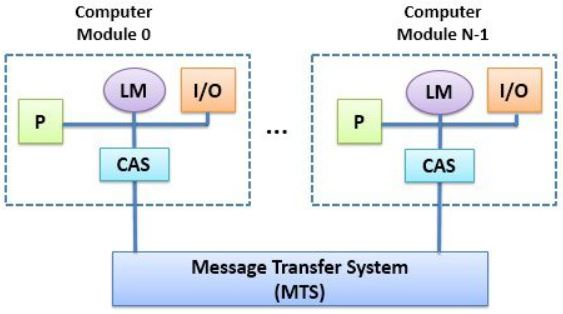
\includegraphics[width=8cm]{../img/loose}
\caption{A loosely coupled multiprocessor system. Each node features it's own memory and IO modules and uses a Message Transfer System to perform inter-node communication. Image source: \cite{preeti_aritra_2017}.}
\label{fig:loose}
\end{figure}
\end{minipage}
\begin{minipage}{0.05\textwidth}\hfill\end{minipage}
\begin{minipage}{0.45\textwidth}
\begin{figure}[H]
\centering
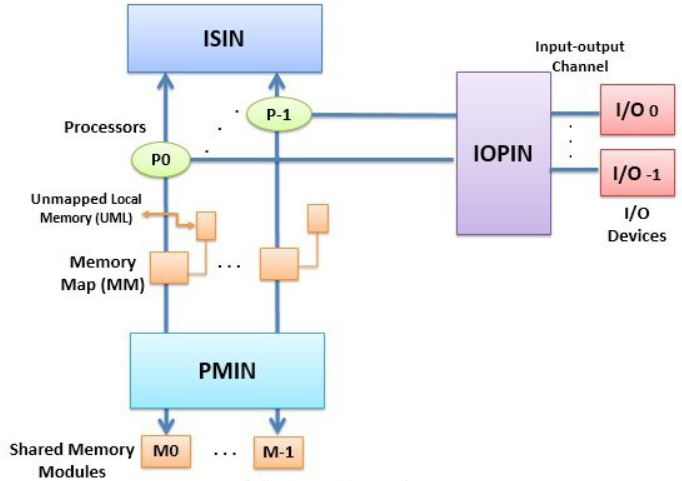
\includegraphics[width=8cm]{../img/tight}
\caption{A tightly coupled multiprocessor system. Nodes are directly connected to memory and IO modules. Image source: \cite{preeti_aritra_2017}.}
\label{fig:tight}
\end{figure}
\end{minipage}
\vspace{0.3cm}

This project will utilise a loosely coupled architecture due to it's easier scalability implementation and my previous experience with the design of single-core processors. Although it will require a scheduler to access the MTS, the experience and knowledge gained from this task will be greatly beneficial for future projects.

\section{Network-on-chip Architectures}
Network-on-chip (NoC) architectures implement on-chip communication mechanisms that are based on network communication  principles, such as routing, switching, and massive scalability \cite{newnoc}. NoC's can generally support hundreds to millions of processing cores.
\cref{fig:noc} shows an example 16-core network-on-chip architecture. 
NoC's can scale to very large sizes while not sacrificing performance because each processor core is able to drive the network rather than needing to wait for a shared bus to become free before doing so.

The greater the number of cores in a network-on-chip design, the greater quality of service (QoS) problems arise. As such, network-on-chip architectures suffer the same problems as networks, such as fairness and throughput \cite{nocfairness}.


\begin{figure}[h]
\centering
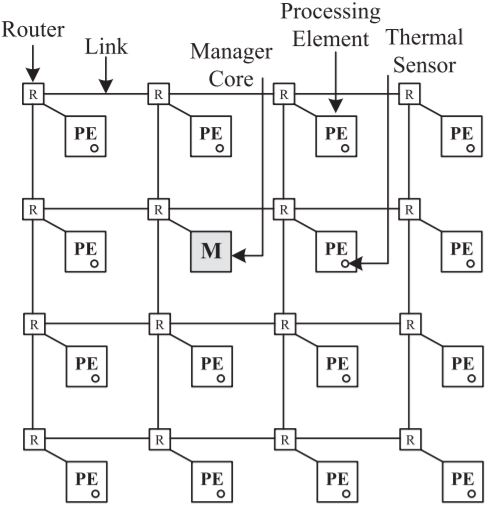
\includegraphics[width=6cm]{../img/noc}
\caption{A multiprocessor network-on-chip architecture with 16 processing nodes. Nodes are connected in a grid formation with routers and links. Image source: \cite{noc}.}
\label{fig:noc}
\end{figure}
